% !TEX TS-program = XeLaTeX

% STYLE

\documentclass[a4paper, 12pt]{article}
\usepackage[left=1in,
		    right=1in,
    		    top=1in,
		    bottom=1in,
		    bindingoffset=0cm]{geometry}
		    \usepackage{array}
\usepackage{float}
\usepackage{graphicx}
\graphicspath{ {./images/} }
\usepackage{subfig}
\usepackage{enumerate}
\usepackage[normalem]{ulem} % underlining
\usepackage{booktabs} % tables
\usepackage[table]{xcolor} % coloring tables
\newcolumntype{L}[1]{>{\raggedright\let\newline\\\arraybackslash\hspace{0pt}}m{#1}} % beautiful column types
\newcolumntype{C}[1]{>{\centering\let\newline\\\arraybackslash\hspace{0pt}}m{#1}}

% LANGUAGE + FONT
		    
\usepackage[english]{babel}
\usepackage[backend=biber,
                     style=unified]{biblatex}
\newcommand{\citeay}[2][]{
   \citeauthor{#2} (\citeyear[#1]{#2})}
\addbibresource{ref.bib}
\usepackage{fontspec}  
\setmainfont{Minion 3}
\usepackage{hyperref}
\hypersetup{
    colorlinks=true,
    linkcolor=black,
    citecolor=black,
    filecolor=black,
    urlcolor=blue,
}

% DRAWING

\usepackage{tikz}
\usepackage{tikz-qtree}
\usetikzlibrary{shapes.geometric}
\usetikzlibrary{trees,arrows}
\usetikzlibrary{positioning}
\usetikzlibrary{matrix}
\usetikzlibrary{tikzmark}
\usetikzlibrary{decorations.shapes}

% LINGUISTICS 

\usepackage{expex}
\usepackage[glossaries]{leipzig}
\makeglossaries
\newleipzig {npst} {npst} {non-past}
\newleipzig {nfin} {nfin} {non-finite}
\newleipzig {nsg} {nsg} {non-singular}
\newleipzig {nzr} {nzr} {nominalizer}
\newleipzig {dim} {dim} {diminutive}
\newleipzig {lat} {lat} {lative case}
\newleipzig {cn} {cn} {connegative}
\newleipzig {ipf} {ipf} {imperfective}

\lingset{numoffset=0ex, aboveexskip=1em, belowexskip=1em}

\title{Moksha dataset}
\author{EGG2023, Novi Sad}
\date{Last updated \today}

\begin{document}
\maketitle

	\section{Basic facts}
	
	European part of Russia, Mordovia Republic and neighbouring regions
	
	\begin{figure}[H]
		\centering
		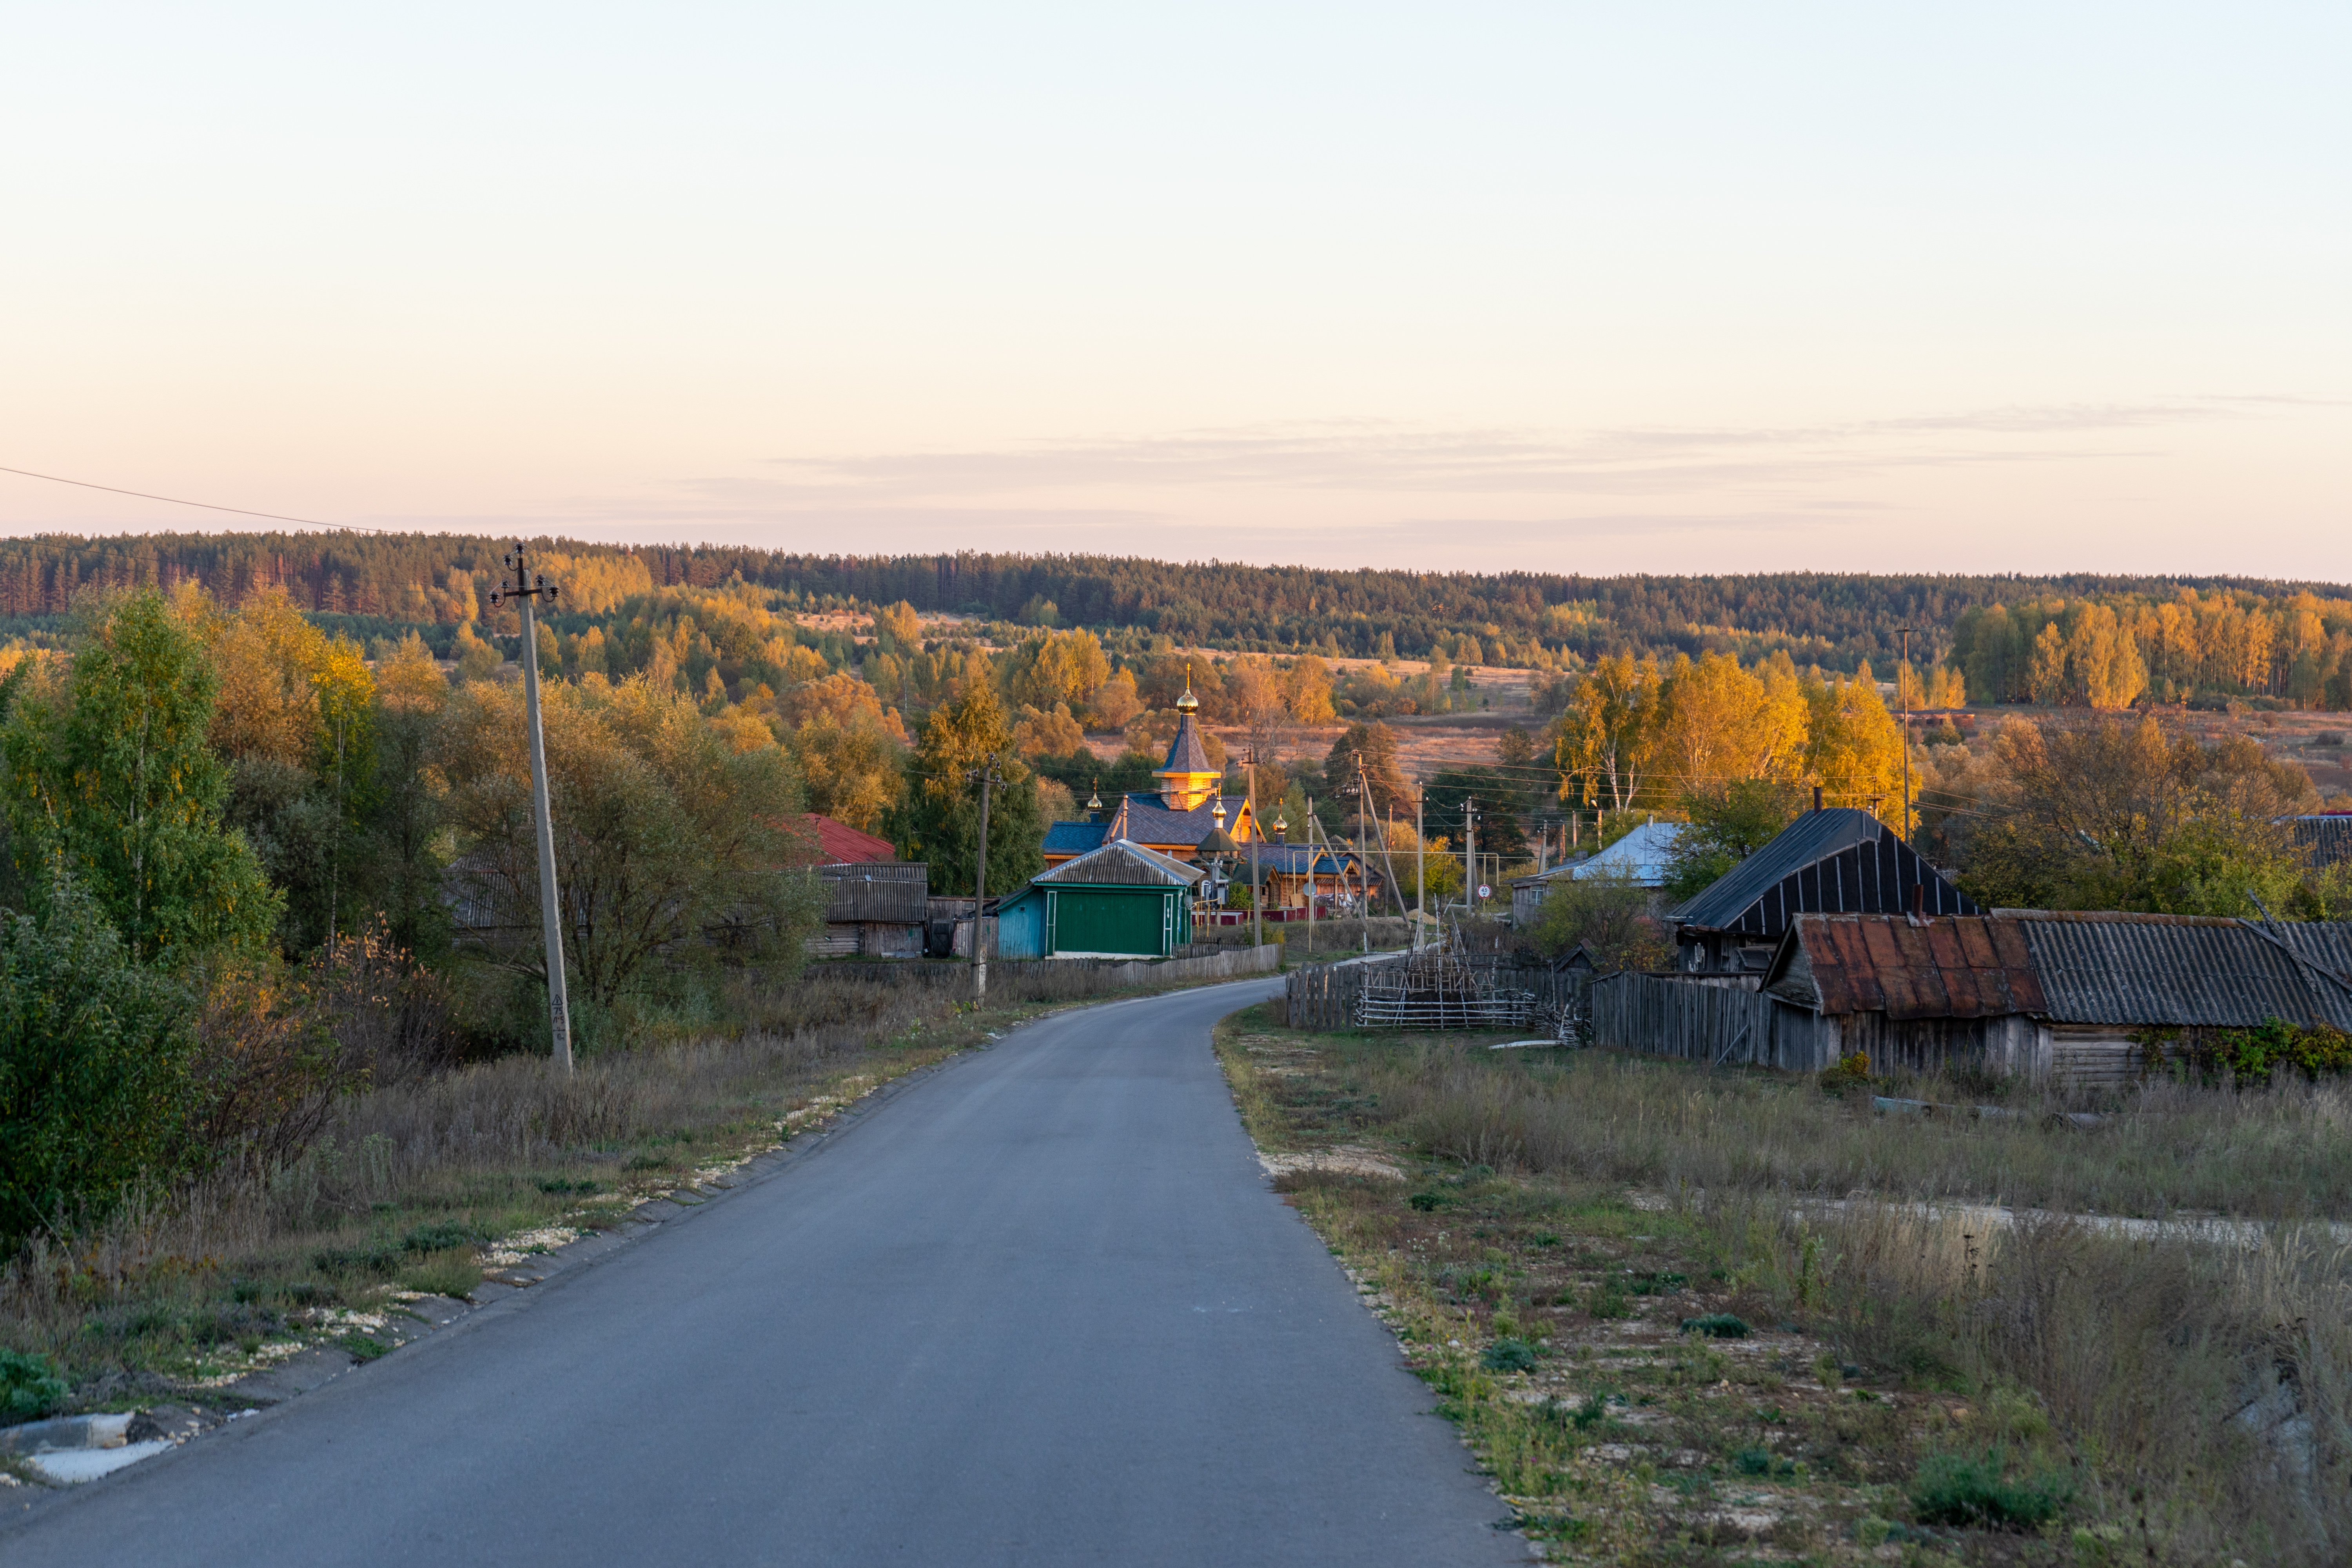
\includegraphics[scale=.125]{mok-beginning}
		\hfill
		\includegraphics[scale=.373]{mok-map}
	\end{figure}
	
	\noindent Vowel and consonant inventories \parencite{kukhto2018}
	
\begin{minipage}[t]{0.45\linewidth}
	\begin{figure}[H]
		\includegraphics[scale=.66]{mok-vowels}
		\hfill
	\end{figure}
\end{minipage}
\hfill
\begin{minipage}[t]{0.45\linewidth}
\begin{table}[H]
\begin{tabular}{lllllll}
\toprule
m   &     & \begin{tabular}[c]{@{}l@{}}n\\ n'\end{tabular}      &                                                       &                                                  &    &     \\
p b &     & \begin{tabular}[c]{@{}l@{}}t d\\ t' d'\end{tabular} &                                                       &                                                  &    & k g \\
    & f v & \begin{tabular}[c]{@{}l@{}}s z\\ s' z'\end{tabular} &                                                       & \begin{tabular}[c]{@{}l@{}}š ž\\ šč\end{tabular} & j̊ & (x) \\
    &     & \begin{tabular}[c]{@{}l@{}}c\\ c'\end{tabular}      &                                                       & č                                                &    &     \\
    &     &                                                     &                                                       &                                                  & j  &     \\
    &     &                                                     & \begin{tabular}[c]{@{}l@{}}r̥ r\\ r̥' r'\end{tabular} &                                                  &    &     \\
    &     & l̥                                                  & l̥'                                                   &                                                  &    &     \\
    &     & l                                                   & l'                                                    &                                                  &    &    
\\
\bottomrule
\end{tabular}
\end{table}
\end{minipage}

	\begin{enumerate}[$\gg$]
		\item Contrastive voicing in stops AND glides
		\item Contrastive palatalisation
		\item /x/ only in loanwords
	\end{enumerate}
	
	\section{Stress}
	
	Based on \citeay{kukhto2018}
	
\begin{table}[H]
\begin{tabular}{llllll}
\toprule
\textbf{Transcription} & \textbf{Gloss}      & \textbf{Transcription} & \textbf{Gloss}        & \textbf{Transcription} & \textbf{Gloss}        \\
\midrule
ˈt'ɛd'ɛ                & `mother'            & kuˈvaka                & `long'                & ˈkijə                  & `who'                 \\
s'im-əˈma              & `drink-{\Nzr}'      & s't'ər'-ˈn'ɛ           & `girl-{\Dim}'         & ˈkud-u                 & `home-{\Lat}'         \\
ˈloman                 & `person'            & ˈsa-tadə               & `come-{\Npst}.{\Tpl}' & uˈfa-j                 & `blow-{\Npst}.{\Tsg}' \\
ˈs't'ər'-n'ə           & `girl-{\Def}.{\Pl}' & ˈjalga                 & `friend'              & ˈmol'-əma              & `go-{\Nzr}'           \\
iˈlɛt                  & `evening'           & ˈmejga                 & `nothing'             & ˈul-ə                  & `be-{\Cn}'       \\
\bottomrule    
\end{tabular}
\end{table}
	
	\section{Glide insertion}
	
	Based on \citeay{kozlov2018} and \href{http://moksha.web-corpora.net}{the Moksha corpus}\\
	
	Schwa-initial suffixes:
	
\begin{minipage}[t]{.3\linewidth}
\ex\label{ex:u1}
	jožu + əl' $\rightarrow$ jožuv-əl' \\`({\Tsg} was) smart-{\Ipf}'
\xe
\end{minipage}
\hfill
\begin{minipage}[t]{.315\linewidth}
\ex\label{ex:a1}
	ava + əl' $\rightarrow$ ava-l' \\`({\Tsg} was a) woman-{\Ipf}'
\xe
\end{minipage}	
\hfill
\begin{minipage}[t]{.33\linewidth}
\ex\label{ex:z1}
	ruz + əl' $\rightarrow$ ruzəl' \\`({\Tsg} was) Russian-{\Ipf}'
\xe
\end{minipage}

\begin{minipage}[t]{.3\linewidth}
\ex\label{ex:u2}
	t'ɛči + ən' $\rightarrow$ t'ɛčij-ən' \\`today-{\Gen}'
\xe
\end{minipage}	
\hfill
\begin{minipage}[t]{.315\linewidth}
\ex\label{ex:a2}
	ava + ən' $\rightarrow$ ava-n' \\`woman-{\Gen}'
\xe
\end{minipage}	
\hfill
\begin{minipage}[t]{.33\linewidth}
\ex\label{ex:z2}
	ruz + ən' $\rightarrow$ ruzən' \\`Russian-{\Gen}'
\xe
\end{minipage}

\begin{minipage}[t]{.3\linewidth}
\ex\label{ex:mono1}
	ši + ən' $\rightarrow$ ši-n' \\`day-{\Gen}'
\xe
\end{minipage}
\hfill
\begin{minipage}[t]{.315\linewidth}
\ex\label{ex:}
	mu + əms $\rightarrow$ mu-ms \\`find-{\Inf}'
\xe
\end{minipage}	
\hfill
\begin{minipage}[t]{.33\linewidth}
\ex\label{ex:mono2}
	vi + əms $\rightarrow$ vi-ms \\`bring-{\Inf}'
\xe
\end{minipage}

	/a/-initial suffixes:

\begin{minipage}[t]{.45\linewidth}
\ex\label{ex:jozu}
	jožu + an $\rightarrow$ jožuvan \\`(I am) smart-{\Fsg}' 
\xe
\end{minipage}
\hfill
\begin{minipage}[t]{.45\linewidth}
\ex\label{ex:vidi}
	vidi + an $\rightarrow$ vidijan \\`(I am) a sower-{\Fsg}' 
\xe
\end{minipage}

\begin{minipage}[t]{.45\linewidth}
\ex\label{ex:mu}
	mu + an $\rightarrow$ mujan \\`(I) find-{\Fsg}' 
\xe
\end{minipage}
\hfill
\begin{minipage}[t]{.45\linewidth}
\ex\label{ex:li}
	li + an $\rightarrow$ lijan \\`(I) fly-{\Fsg}' 
\xe
\end{minipage}		

\begin{minipage}[t]{.45\linewidth}
\ex\label{ex:jaka}
	jaka + at $\rightarrow$ jakat \\`(you) go-{\Ssg}'
\xe
\end{minipage}
\hfill
\begin{minipage}[t]{.45\linewidth}
\ex\label{ex:atya}
	at'ɛ + an $\rightarrow$ at'an \\`(I am) an old man-{\Fsg}' 
\xe
\end{minipage}	

\begin{minipage}[t]{.45\linewidth}
\ex\label{ex:sa}
	sa + an $\rightarrow$ sajan \\`(I) come-{\Fsg}' \\ \parencite[p. 57]{kozlov2018}
\xe
\end{minipage}
\hfill
\begin{minipage}[t]{.45\linewidth}
\ex\label{ex:shna}
	šna + an $\rightarrow$ šnajan \\`(I) praise-{\Fsg}'
\xe
\end{minipage}	

	\section{Loanword data}
	
	All of the following examples illustrate how loanwords (primarily Russian) behave wrt. stress and glide insertion. 
	
\begin{minipage}[t]{.45\linewidth}
\ex\label{ex:krushka}
	ˈkruška `cup'
\xe
\end{minipage}
\hfill
\begin{minipage}[t]{.45\linewidth}
\ex\label{ex:kniga}
	ˈkniga `book' 
\xe
\end{minipage}
	
\begin{minipage}[t]{.3\linewidth}
\ex\label{ex:lw1s}
	žuˈri + ən' $\rightarrow$ žuri-n' \\`jury-{\Gen}' 
\xe
\end{minipage}
\hfill
\begin{minipage}[t]{.3\linewidth}
\ex\label{ex:lw2s}
	ˈsoči + ən' $\rightarrow$ soči-n' \\ `Sochi-{\Gen}' 
\xe
\end{minipage}	
\hfill
\begin{minipage}[t]{.3\linewidth}
\ex\label{ex:lw3s}
	li + ən' $\rightarrow$ li-n' \\ `Li-{\Gen}'
\xe
\end{minipage}
	
	\section{Questions to consider}
		
\begin{enumerate}[$\gg$]
	\item Formulate the stress rule for native Moksha words. What does the stress depend on?
	\item Is stress weight-sensitive?
	\item How are loanwords different?
	\item In what contexts does glide insertion happen?
	\item How are /a/-initial suffixes different from the schwa-initial ones?
\end{enumerate}
		
%\begin{enumerate}[$\gg$]
%	\item 
%\end{enumerate}

	\section*{Glossing abbreviations}
	
\printglossaries
	
\printbibliography

	\begin{figure}[H]
		\centering
		\includegraphics[scale=.166]{mok-end}
	\end{figure}

\end{document}